\documentclass[
12pt,
a4paper,
%BCOR=10mm, % boundary correction, lost in binding
bibliography=totoc,
captions=nooneline, % one line caption left aligned just like multiline captions
numbers=noenddot,
twoside]{scrbook}
\addtokomafont{caption}{\small}
\setkomafont{captionlabel}{\sffamily\bfseries}
\setcapindent{0em} % save space with multiline captions; default is \setcaphanging
\setlength{\textheight}{650pt} % keep inner/outer margins, but make text "taller", default 598pt.
\setcounter{secnumdepth}{3}
\setcounter{tocdepth}{3}

\usepackage[T1]{fontenc}
\usepackage[utf8]{inputenc}

% times new roman and matching math font
\usepackage{libertine}
\usepackage{newtxmath}

\usepackage{bm,amssymb,amsfonts,amsmath}  % bold math symbols, AMStex

\usepackage{booktabs}
\usepackage[svgnames]{xcolor}
\usepackage{graphicx}
% trailing slash is crucial!
\graphicspath{
  {./}
  {./figures/}
}

\usepackage{hyperref}
\synctex=1 % cross correlate PDF viewer and editor

\usepackage[numbers,sort&compress]{natbib}
\usepackage{parskip}
\usepackage[colorinlistoftodos]{todonotes} % Use 'disable' to remove todos in final version

\newcommand{\bat}{{\sc BAT}}
\newcommand{\Root}{{\sc ROOT}}

\newcommand{\versionno}{1.1.0-DEV}

\newcommand{\version}{version~\versionno}
\newcommand{\Version}{Version~\versionno}

\newcommand{\code}[1]{\texttt{#1}}

\newcommand{\dan}[1]{{\todo[color=red]{Dan: #1}}}
\newcommand{\fred}[1]{{\todo[color=orange]{Fred: #1}}}
\newcommand{\inbat}[1]{{\todo[color=Salmon!40,inline]{#1}}}
\newcommand{\batnote}[1]{{\todo[color=Salmon!40,noline]{#1}}}

% references to ...
\def \refchap#1{Chapter~\ref{cha:#1}}
\def \refeq#1{(\ref{eq:#1})}
\def \refsec#1{Section~\ref{sec:#1}}
\def \reffig#1{Figure~\ref{fig:#1}}
\def \reftab#1{Table~\ref{tab:#1}}

% syntax highlighting
\usepackage{listings}
\definecolor{mygray}{rgb}{0.4,0.4,0.4}
\definecolor{mygreen}{rgb}{0,0.8,0.6}
\definecolor{myorange}{rgb}{1.0,0.4,0}
\lstset{
  backgroundcolor=\color{black!5}, % set backgroundcolor
  language=c++,
  gobble=0,
  commentstyle=\itshape\color{purple!80},
  breaklines=true,
  basicstyle=\ttfamily\color{black}\scriptsize,
  frame=single,
  % identifierstyle=\color{blue},
  keywordstyle=\color{myorange},
  numberstyle=\tiny\color{mygray},
  showspaces=false,
  showstringspaces=false,
  stringstyle=\color{myorange},
  tabsize=4,
}
\lstnewenvironment{cxxcode}
{}
{}
\newcommand{\cxxin}[1]{\lstinline{#1}}

% math
\newcommand{\cond}{\,|\,}
\newcommand\rmdx[1]{\mbox{d}#1\,} % differential
\newcommand{\scath}{\theta} % scalar parameter
\newcommand{\vecth}{\bm{\theta}} % vector parameter

% --------------------------------------------------------
% document
% --------------------------------------------------------
\begin{document}

% --------------------------------------------------------
% title
% --------------------------------------------------------

\thispagestyle{empty}

\begin{figure}

\includegraphics[scale=0.25]{bat}
\end{figure}

\vspace*{1cm}

\begin{center}


{\Large \bat{} Manual}
\\

\vspace{1cm}

{\large \bat\ \version}

\end{center}

\thispagestyle{empty}

\vfill

\begin{center}
\today
\end{center}

\pagebreak

% --------------------------------------------------------
% table of contents
% --------------------------------------------------------

\thispagestyle{empty}

\enlargethispage{2cm}

\tableofcontents{}

% \listoftodos

\mainmatter

\section*{Overview}

\fred{what is this for, web page, reference guide, github, teaser}

The purpose of this document is to introduce the Bayesian Analysis
Toolkit (BAT). \fred{Say in two sentences what BAT is for.} For a
quick tutorial covering the basic features, jump directly to
\refsec{basics}.

\subsection*{Structure of this document}

We give a brief introduction of the Bayesian approach to statistics in
\refsec{Bayes} and describe the core algorithm of \bat{}, Markov chain
Monte Carlo, in \refsec{MCMC}. Further sections describe other parts
of \bat{} and advanced features.

\subsection*{Further help}

Please visit our home page at \url{http://mpp.mpg.de/bat} for an
overview of documentation and activities around \bat{}.

This document is meant to is quickly enable to you to find your way
around \bat{}. We describe the common workflow and explain how to
solve some not-so-common tasks. To keep the size of this document
manageable, we refer you to the
\href{http://mpp.mpg.de/bat/docs/refman/latest/}{online reference
  guide} in which all classes, methods etc. are documented.

If you find a problem with the code, the preferred method is to create
a new issue at \url{https://github.com/bat/bat/issues}. If you provide
some code for us to reproduce the problem, we can help you much
faster.

For general questions or comments, contact the developers at
\href{mailto:bat@mpp.mpg.de}{bat@mpp.mpg.de}.

\part{Basics}
\chapter{Tutorial} \label{sec:basics}

Goal of this section is that you can read and test as you go along, and end up with functioning code.

\section{Installation instructions}

Detailed instructions for downloading and installing BAT are in the
\verb|INSTALL.md| file that comes with the \bat\ source distribution. The
latest version is available online at
\url{https://github.com/bat/bat/blob/master/INSTALL.md}.

\fred{Add link to instructions in appendix as per \href{https://github.com/bat/bat/issues/145}{\#145}}

\section{Non-code parts of BAT}
\dan

bat-project, bat-config
\begin{cxxcode}
int main() {
  std::string s = "Hello";
  return 0;
}
\end{cxxcode}

\section{Absolutely necessary requirements of your model}
\dan

Parameters, LogLikelihood, some form of setting a prior.

\section{Running the analysis}
\dan

Functions to call. How to output. Basic tuning. How to interpret runtime log output \& trouble shooting (nonconvergence, poor efficiencies). How to interpret summary log output.

\section{Plots}
\dan

Interpreting the basic output: marginals; parameters; knowledge update; correlation matrix.

Options for the different output types.

\chapter{Bayesian Statistics} \label{sec:Bayes}

\fred{Just introduce terminology and symbols. Refer to other book:
  Jaynes, Gelman. Which questions are of interest, which can be
  answered more easily with \bat, this includes goodness of fit with p
  values which is not exactly Bayesian}

In this chapter, we give a concise and necessarily incomplete overview
of Bayesian statistics. Our intention is to cover the bare minimum and
introduce those quantities that appear in \bat. There is vast
literature on the subject; we refer the reader to the books
\cite{jaynes_probability_2003, hartigan_bayes_1983, sivia_data_2006,
  mackay_information_2003, dagostini_bayesian_2003,
  kendall_kendalls_2004} for a comprehensive overview.

\section{Basic terminology} \label{sec:basic-terminology}

Bayesian statistics is a framework for quantitative inductive or
plausible reasoning; i.e., the optimal processing of incomplete
information. The basic idea is to associate a degree of belief to
logical propositions; e.g., the mass of the Higgs boson is 125
GeV. From fundamental axioms about reasoning, one can then show that
the calculus of degree of belief is simply the ordinary calculus of
probability theory; see~\cite{jaynes_probability_2003} for a thorough
discussion. Deductive reasoning is included as the limiting case in
which the degree of belief is either 0 or 1.

From now on, we will use the symbol $P(A)$ to denote both the \emph{degree
of belief} in proposition $A$ and the \emph{probability} of $A$. In our
applications below, $A$ is often one value out of a continuum, so we
use $P(A)$ also to denote the \emph{probability density} of $A$.  The
\emph{conditional probability} of $A$ given $B$ is $P(A \cond B)$.

The two central tasks of the natural sciences are to learn about
nature from data and to make predictions for (future) experiments. A
re\emph{model} $M$ is a proxy for all discrete pieces of information relevant
to calculating the degree of belief. The model can contain \emph{parameters}
$\vecth$ that can take on values in a continuum, perhaps subject to
constraints as for example $\scath_1 \geq 0$. Bayesian reasoning
provides an update rule to adjust the degree of belief based on new
information available in the form of \emph{observed data} $D$. This update
rule is the celebrated \emph{Bayes' theorem}
\begin{align}
  \label{eq:bayes-thm}
  \boxed{  P(\vecth \cond D, M) \propto P(D|\vecth, M) P(\vecth \cond M)
  }
\end{align}
$P(\vecth \cond M)$ is the \emph{prior density}, $P(D|\vecth, M)$ is
called the \emph{probability of the data} when treated as a function
of $D$, and known as the \emph{likelihood} when considering the
dependence on $\vecth$, for fixed $D$. The model-dependent
normalization constant is known as the \emph{evidence} or
\emph{marginal likelihood}:
\begin{equation}
  \label{eq:evidence}
  Z = \int \rmdx{ \vecth} P(D|\vecth, M) P(\vecth \cond M).
\end{equation}
Finally, the left-hand side of \eqref{eq:bayes-thm}, $P(\vecth | D,
M)$, is the \emph{posterior density}. Prior and posterior (``density''
is usually omitted) represent the state of knowledge about the
parameter $\vecth$ before and after seeing the data. Note that
$\vecth$ appears on opposite sides of ``|'' in $P(D|\vecth,M)$ and
$P(\vecth|D,M)$. That's why Bayes' theorem is also known as the
theorem of \emph{inverse probability}.

\subsection{Marginalization} \label{sec:marginalization}

Suppose there are two parameters, $\vecth = (\scath_1, \scath_2)$, and
$\scath_1$ is the \emph{parameter of interest} whereas $\scath_2$ is a
\emph{nuisance parameter}. In Bayes' theorem, there is no fundamental
distinction between parameters of interest and nuisance parameter,
they are all just parameters. But often the goal of the analysis is to
extract the posterior of $\scath_1$ while $\scath_2$ is only needed at
an intermediate stage; for example in order to correctly model the
measurement process of $D$. From the joint posterior $P(\scath_1,
\scath_2 | D)$, we compute the \emph{marginalized} posterior and can
remove the dependence on $\scath_2$ by integration
\begin{align}
  \label{eq:marginal}
  P(\scath_1 | D) = \int \rmdx{\scath_2} P(\scath_1, \scath_2 | D).
\end{align}

\subsection{Model comparison} \label{sec:model-comparison}

If there is only a single model under consideration, and no potential for
cconfusion, the model label $M$ is implied and usually omitted from the
equations. But suppose that there are two competing models, $M_1, M_2$, with
parameters $\scath_{1,2}$, that quantitatively predict the outcome $D$ of an
experiment. The task is to find the model with the higher degree of
belief. Using Bayes' theorem, the \emph{posterior odds} of the models are easily
found as
\begin{equation}
  \label{eq:post-odds}
  \frac{P(M_1|D)}{P(M_2|D)}
   = B_{12}  \cdot  \frac{P(M_1)}{P(M_2)},
\end{equation}
 where the \emph{Bayes factor} of $M_1$ versus $M_2$, $B_{12}$, is just the ratio
of the evidences
\begin{equation}
  \label{eq:Bayes-factor}
  B_{12}= \dfrac{P(D|M_1)}{P(D|M_2)} = \frac{Z_1}{Z_2}
  = \frac{\int \rmdx{\vecth_1} P(D|\vecth_1, M_1) P(\vecth_1, M_1)}
  {\int \rmdx{ \vecth_2} P(D|\vecth_2, M_2) P(\vecth_2, M_2)}
\end{equation}
The \emph{prior odds} $P(M_1)/P(M_2)$ represent the relative degree of belief
in the models, independent of the data.
% The data are accounted for in the Bayes factor.
The Bayes factor quantifies the relative shift of degree of belief
induced by the data. In general, $\dim \vecth_1 \ne \dim \vecth_2$,
and without loss of generality let $\dim \vecth_1 < \dim
\vecth_2$. The Bayes factor automatically penalizes $M_2$ for its
larger complexity, as the prior mass is spread out over a
higher-dimensional volume. However, this can be compensated if the
likelihood $P(D|\vecth_2, M_2)$ is significantly higher in regions of
reasonably high prior density; i.e. the Bayes factor implements
Occam's razor the simplest model that describes the observations is
preferred.

\section{Goodness of fit} \label{sec:goodness-fit}
In the Bayesian approach, there is, however, no straightforward answer to the
following question: if there is only one model at hand, how to decide if that
model is sufficient to explain the data, or if the search for a better model
needs to continue?  The standard procedure to tackle this problem of evaluating
the \emph{goodness of fit} is explained in \fred{expand}

\section{Representation in BAT} \label{sec:representation-bat}

In \bat, a model $M$ is represented as a C++ subclass of
\code{BCModel}. The crucial parts are to define the likelihood $P(D
\cond \vecth, M)$, the prior $P(\vecth \cond M)$, and the parameters
$\vecth$. From these quantities, \bat{} can compute the posterior
$P(\vecth \cond D, M)$. To avoid numerical overflow, \bat{} operates
on the log scale whenever possible.  The key methods a user has to
implement are
\fred{Perhaps mention \bat{} in framed insets right where terms are introduced.}

\begin{cxxcode}
virtual double LogLikelihood(const std::vector<double>& params)
virtual double LogAPrioriProbability(const std::vector<double>& params)
\end{cxxcode}
\fred{The whole section might go somewhere else where users find it more
  easily. I fear it would get lost here} The parameter values are
passed in simply as numbers to likelihood and prior, all parameters
are assumed to be real and continuous. Discrete parameters are not
supported. The support of $\vecth$ is a hyperrectangle whose bounds
are given by the bounds of the individual parameters when added to the
model with
\begin{cxxcode}
bool AddParameter(const std::string& name, double min, double max, const std::string& latexname = "", const std::string& unitstring = "")
\end{cxxcode}
The optional \cxxin{latexname} and \cxxin{unitstring} are used only
for labeling plot axes; it's intended usage is to pretty up plots. For
example, a parameter \cxxin{theta} representing a time measured in
seconds is defined as
\begin{cxxcode}
AddParameter("theta", 0, 1, "#theta", "s");
\end{cxxcode}
and whenever \cxxin{theta} appears on the x axis of a plot, it will
appears as ``$\theta$ [s]''. Note that the plots are created with \Root,
so the \cxxin{latexname} has to be in \Root{} syntax which is mostly
 \LaTeX{} syntax with ``\textbackslash" $\to$ ``\#''.

\chapter{Markov chain Monte Carlo} \label{sec:MCMC}

\fred{workhorse of BAT. mention Metropolis algorithm, role of proposal function, different choices in bat, why it has to be adapted in prerun. What else happens in prerun:R value and convergence checking. Mention that samples are correlated, chains can get stuck if model wrong/poor.}

\section{Motivation}\label{sec:mcmc-motivation}

The reason that \bat{} exists is that nearly any Bayesian analysis
these days is too complicated to be handled analytically. To address
typical questions like
\begin{enumerate}
  \item What is known about a single parameter taking into account
  the uncertainty on all other parameters?
  \item How are parameters correlated?
\end{enumerate}
one needs to be able to compute and visualize 1D and 2D \emph{marginal distributions}; cf. \refsec{marginalization}. These are defined as integrals over the posterior; for  example in 2D
\begin{align}
  \label{eq:mcmc-marginal}
  P(\theta_1, \theta_2 \cond D) = \int \prod_{i \ne 1,2} \rmdx{\theta_i} P(\vecth \cond D).
\end{align}
When the number of parameters grows, the only feasible algorithms to
perform the integration are Monte Carlo methods; i.e., methods based
on random numbers.

The key ingredient in \bat{} is an implementation of the Metropolis
algorithm to create a Markov chain; i.e. a sequence of (correlated)
samples from the posterior. We use the shorthand MCMC for Markov chain
Monte Carlo.

\section{Foundations}\label{sec:mcmc-foundations}

Efficient MCMC algorithms are the topic of past and current
research. This section is a concise overview of the general idea and
the algorithms available in \bat. For a broader overview, we refer the
reader to the abundant literature; e.g., \fred{Robert+Casella, MCMC
  handbook}.

In \bat{}, there are several variants of the random-walk Metropolis Hastings algorithm available. The basic idea is captured in the 2D example shown in \reffig{random-walk-idealized}. Given an initial point $x_0$, the Metropolis algorithm produces a sample in each iteration $t=1 \dots$ as follows:

\begin{enumerate}
  \item Propose a new point $y$
  \item Generate a number u from the uniform distribution on [0,1]
  \item Set $x_{t} = y$ if $ u < \frac{P(y \cond D)}{P(x_{t-1} \cond D)}$
  \item Else stay, $x_t = x_{t-1}$
\end{enumerate}

\begin{figure}[ht]
  \centering
  % \includegraphics[width=0.8\textwidth]{random-walk}
  \Large
  \def\svgwidth{1\columnwidth}
  \input{figures/random-walk.pdf_tex}
  \caption{2D random walk. The chain begins in the lower left
    corner. Rejected moves are indicated by the dashed arrow, accepted
    moves are indicated by the solid arrow. The circled number is the
    number of iterations the chain stays at a given point $\vecth = (\theta_1, \theta_2)$.}
  \label{fig:random-walk-idealized}
\end{figure}

\section{Convergence}\label{sec:convergence}
\fred{mixing, burn in, R value, multimodal problems}

\section{Implementation in BAT}

Implementing the Metropolis algorithm, one has to decide on how to
propose a new point based on the current point. For a random walk,
this is given by the \emph{proposal distribution} $q(y \cond x)$. The
main difference between MCMC algorithms is typically given by
different choices of $q$. The Metropolis algorithm doesn't specify
 which $q$ to choose, so we can tune it according to our needs.

In \bat{}, the proposal is \emph{symmetric} around the current point
\begin{align}
  q(y \cond x) = q(x \cond y).
\end{align}

There are two stages


\fred{Overall scheme: prerun and main run, adaptation in the prerun}

We offer two variants termed \emph{factorized} and \emph{multivariate}.

\subsection{Factorized proposal}\label{sec:factorized}

\inbat{Factorized was the default and only choice prior to v1.0 and continues to be available.}

\fred{how to activate it}

The factorized proposal in $d$ dimensions is a product of 1D
proposals. We sequentially vary one parameter at a time and complete
one iteration of the chain once a new point has been proposed in every
direction. This means the chain attempts to perform a sequence of
axis-aligned moves in one iteration.

\fred{Easiest to understand would be pseudocode}

Each 1D proposal is a Cauchy or Breit-Wigner function centered on the
current point. The scale parameter is adapted in the prerun to achieve
an acceptance rate in a given range that can be adjusted by the
user. Note that there is a separate scale parameter in every dimension.

This means the posterior is called $d$ times in every iteration. Since
the acceptance rate\fred{to define before} is typically different from
zero or one, the factorized proposal typically generates a new point
in every iteration that differs from the previous point in some but
not all dimensions.

\subsection{Multivariate proposal}\label{sec:multivariate}

\batnote{New in v1.0} Changing all $d$ parameters at once within one
iteration is an all-or-nothing approach. If the proposed move is
accepted, all parameters have changed for the price of a single
evaluation of the posterior. If the move is rejected, the new point is
identical to the old point and the chain does not explore the
parameter space.

We implement the adaptive algorithm by~\cite{Haario:2001}. In brief,
the proposal is a multivariate Gaussian or Student's t distribution
whose covariance is learned from the covariance of samples in the
prerun. An overall scale factor is tuned to force the acceptance rate
into a certain range.

\fred{Pseudocode}

\subsection{Comparison}\label{sec:proposal-comparison}

Comparing the factorized propoasal to the multivariate proposal, we
generally recommend the multivariate for most purposes. B

Use the factorized proposal if you can speed up the computation of the
posterior if you know that some parameters did not change. This can be
useful if the computation is expensive from some but not all
parameters.

\chapter{Non-MCMC parts of BAT}

\section{Integration}
\fred{Users are confused what integration is needed for: state clearly that cuba is only for evidence. But marginalization can be done by something else than MCMC. We have grid methods implemented}


\section{Optimization}
\fred{afterburner or stand-alone, minuit, simulated annealing. How to get results from Minuit run}

\chapter{Accompanying Models}

\section{Using BAT's native data structures}

\section{base}
\section{Efficiency Fitter}
\section{Graph Fitter}
\section{Histogram Fitter}

\section{mtf}
\fred{Kevin should give advice here. Need channels, processes, goodness of fit}

\pagebreak
\part{Advanced BAT}

\chapter{Structure of the code}
\fred{A few paragraphs, what inherits from what, parameter handling,
  pointer to the reference guide where more info is available such
  that one can click directly on classes etc.}

\chapter{ModelManager for Model Comparison}
\fred{can work on same data set but not required}


\chapter{Defining your own factorized prior}
\dan

\chapter{Sharing / Loading samples}
\dan{describe that files can be checked during prerun if \#136 is merged}

\chapter{Uncertainty propagation} \label{cha:uncert-prop}
\fred{How to compute BCObservables, example in ratio model. Plotting of BCObservables, example: 1 parameter changing, evaluate function at 20 points}

\chapter{Performance / Threading / User's attention to thread-safety}

\fred{tips taken over from old manual and expanded. Some advice when it can provide speed up, clearly state that only the MCMC is with threads but synchronization is a bottle neck for fast posteriors}

\chapter{Output}
\section{Logging}
\section{Textual summary}
\fred{summary output, latex tables}
\section{Graphical summary}
\fred{BCSummaryTool}

\chapter{Examples}

\fred{how to run them, suggest to modify them}

\chapter{Validation}

\fred{make check, unit test, performance test suite, building on various platforms}

\chapter{Troubleshooting or FAQ}

\chapter{Tuning MCMC}

\fred{
 scales dimish to zero, chains stuck: error in the model, parameter ranges inappropriate
}

\bibliographystyle{plain}
\bibliography{references.bib}

\end{document}

% Local Variables:
% compile-command:"rubber --pdf -W refs -W misc manual"
% End:
